\section{Visão geral da arquitetura}

A arquitetura apresentada nesta etapa representa o fluxo de dados necessário
para utilizar o Vulkan na implementação de UV Mapping Dinâmico e Procedural.
O objetivo é relacionar os recursos da API com as etapas de processamento
responsáveis pela transformação e utilização das coordenadas de textura.

A Figura~\ref{fig:pipeline-vulkan} apresenta uma visão geral da arquitetura.
Os recursos em azul representam dados e recursos utilizados pela aplicação,
os elementos em verde representam etapas de processamento e shaders, os
elementos em laranja representam mecanismos de sincronização e os elementos
em roxo representam o Render Pass e seus attachments. Os elementos em
amarelo destacam especificamente as operações relacionadas ao UV Mapping.

\begin{figure}[H]
    \centering
    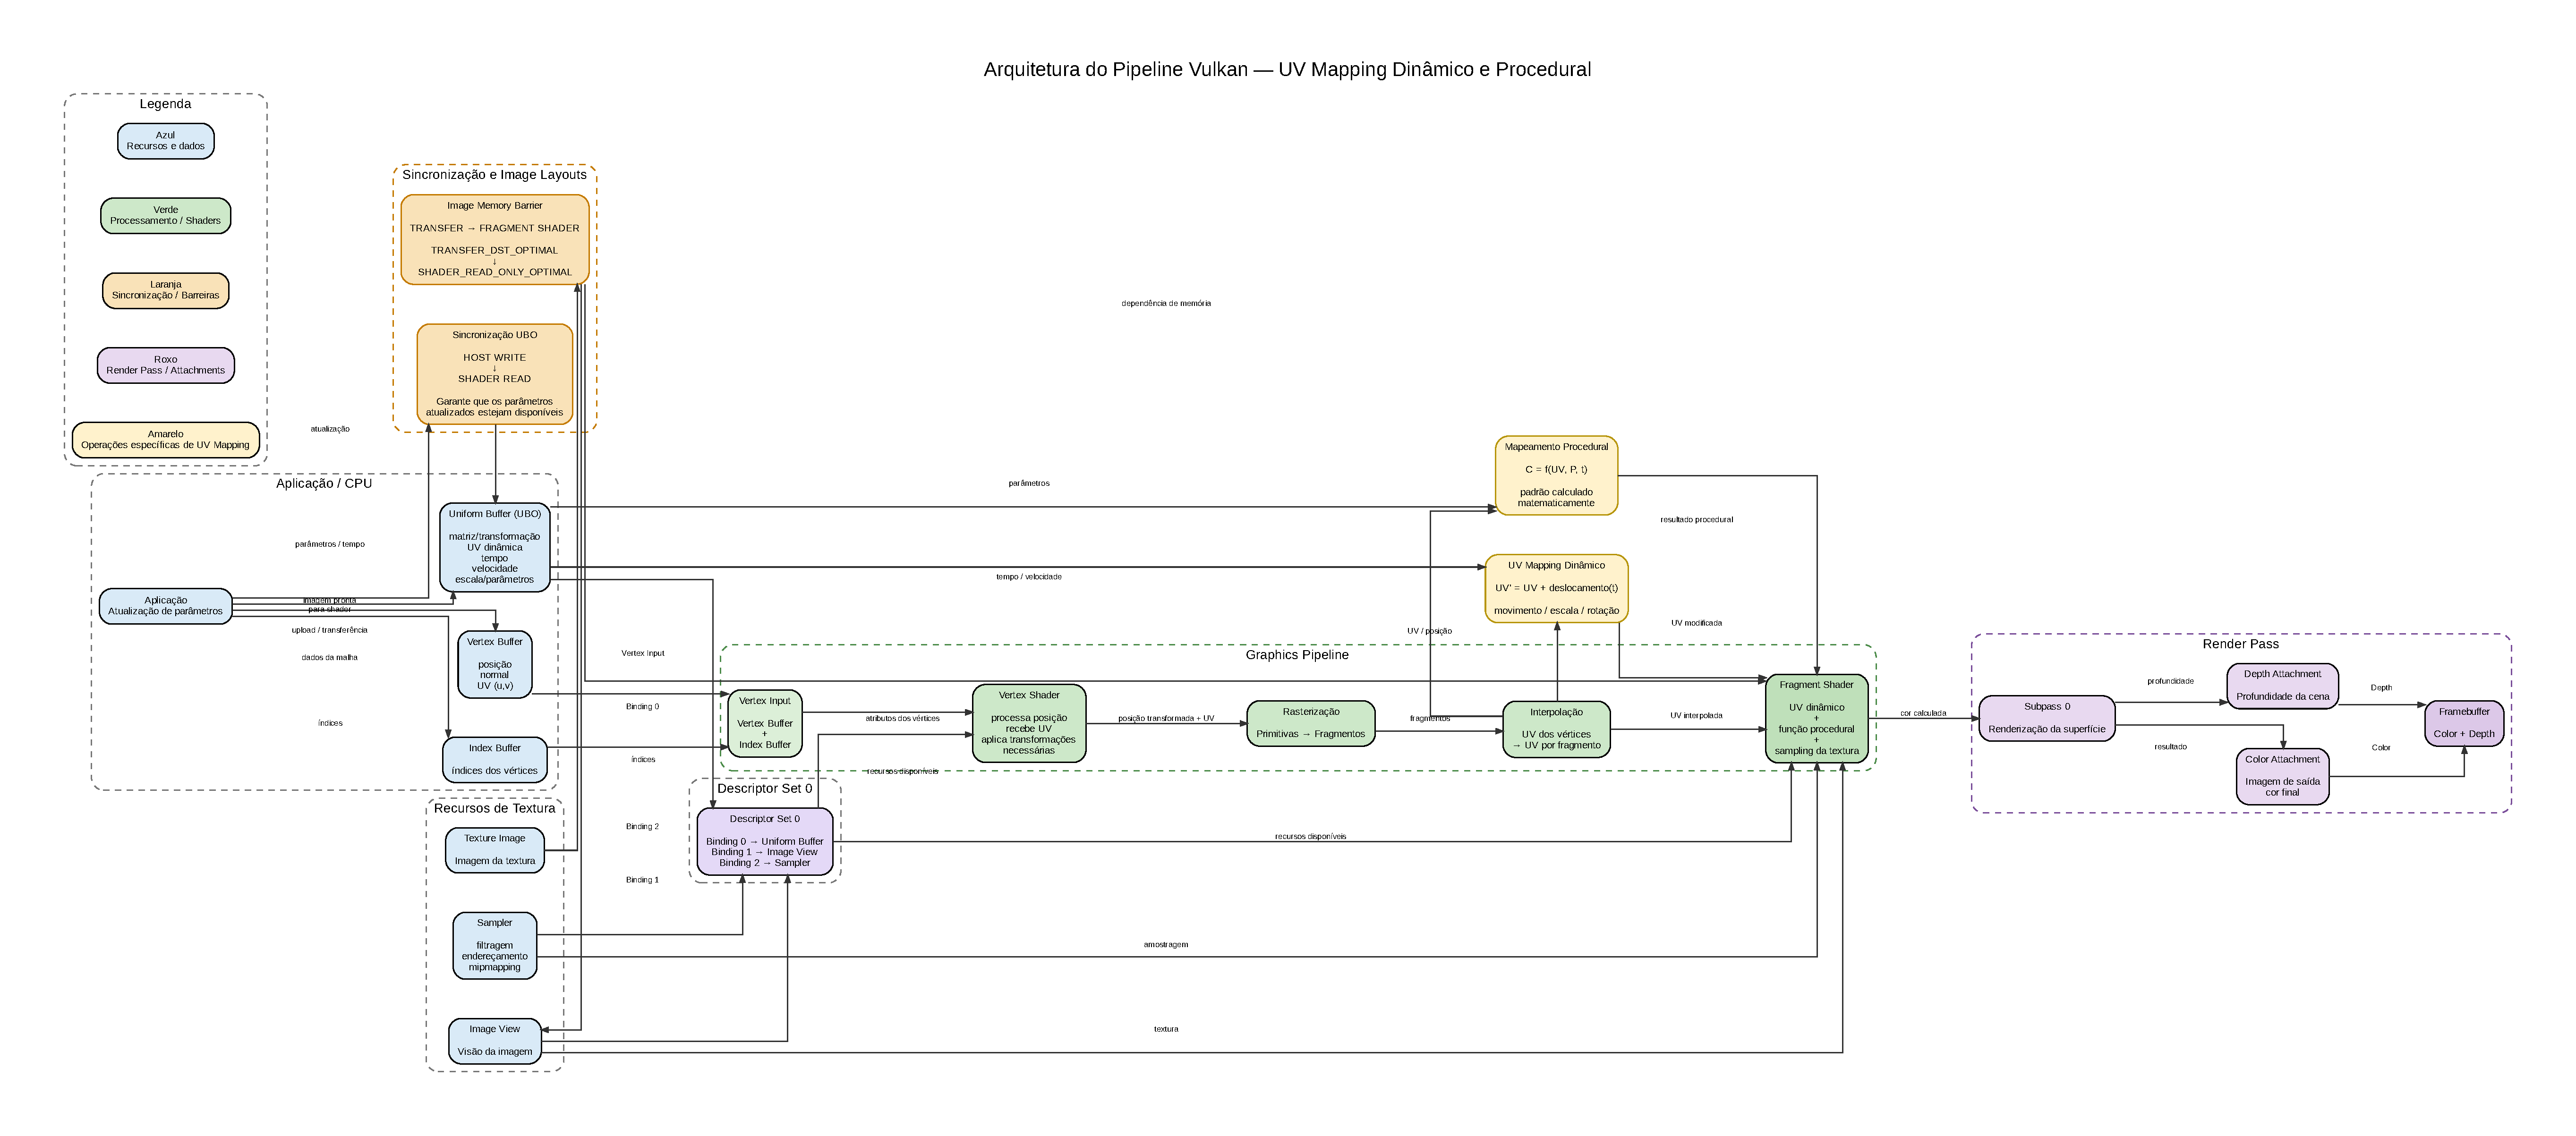
\includegraphics[
        width=\textwidth
    ]{diagrama/pipeline_vulkan.pdf}
    \caption{Arquitetura do pipeline Vulkan aplicada ao UV Mapping Dinâmico e Procedural.}
    \label{fig:pipeline-vulkan}
\end{figure}

\section{Fluxo de dados}

O processamento começa na aplicação, responsável por fornecer os dados da
malha e os parâmetros necessários para a renderização. O Vertex Buffer
armazena os atributos dos vértices, incluindo posição, normal e coordenadas
UV. O Index Buffer armazena os índices utilizados para formar as primitivas
da malha.

Além desses dados, a aplicação pode atualizar parâmetros durante a execução,
como tempo, velocidade de deslocamento, escala e outros parâmetros utilizados
pela técnica. Esses valores são armazenados em um Uniform Buffer (UBO) e
disponibilizados aos shaders por meio do Descriptor Set.

O fluxo principal pode ser resumido como:

\begin{center}
\begin{tabular}{c}
\textit{Vertex Buffer + Index Buffer}
$\rightarrow$
\textit{Vertex Input}
$\rightarrow$
\textit{Vertex Shader}
\\[0.2cm]
$\rightarrow$
\textit{Rasterização}
$\rightarrow$
\textit{Interpolação UV}
$\rightarrow$
\textit{Fragment Shader}
\\[0.2cm]
$\rightarrow$
\textit{Color Attachment}
$\rightarrow$
\textit{Framebuffer}
\end{tabular}
\end{center}

Durante esse processo, as coordenadas UV são transportadas pelos estágios do
pipeline e podem ser modificadas para produzir o efeito dinâmico ou
procedural desejado.

\section{Vertex Buffer e Index Buffer}

O Vertex Buffer contém os dados associados aos vértices da superfície
renderizada. Para esta técnica, são relevantes principalmente a posição do
vértice e suas coordenadas UV. As coordenadas UV indicam a posição
correspondente na textura bidimensional.

O Index Buffer contém os índices utilizados para definir a ordem dos
vértices que formam as primitivas. Dessa maneira, a geometria pode ser
descrita sem a necessidade de repetir todos os atributos dos vértices.

Esses buffers são utilizados no estágio de entrada do pipeline e fornecem os
dados que serão processados pelo Vertex Shader.

\section{Uniform Buffer}

O Uniform Buffer é utilizado para armazenar valores que podem ser atualizados
pela aplicação e utilizados pelos shaders. No contexto do UV Mapping
Dinâmico e Procedural, podem ser armazenados parâmetros como tempo,
velocidade de deslocamento, escala e parâmetros utilizados pelas funções
procedurais.

Um exemplo é o deslocamento dependente do tempo:

\begin{equation}
u' = u + v_u t,
\qquad
v' = v + v_v t.
\end{equation}

Nesse caso, $v_u$ e $v_v$ representam velocidades de deslocamento e $t$
representa o tempo. A aplicação atualiza esses valores e o shader os utiliza
durante a renderização.

\section{Descriptor Set e Bindings}

O Descriptor Set 0 organiza os recursos utilizados pelos shaders. Na
arquitetura apresentada, são considerados três bindings principais.

\begin{table}[H]
    \centering
    \caption{Organização do Descriptor Set 0.}
    \label{tab:descriptor-set}
    \begin{tabular}{c l l}
        \toprule
        \textbf{Binding} & \textbf{Recurso} & \textbf{Finalidade} \\
        \midrule
        0 & Uniform Buffer & Parâmetros dinâmicos e procedurais \\
        1 & Image View & Acesso à imagem da textura \\
        2 & Sampler & Filtragem e endereçamento \\
        \bottomrule
    \end{tabular}
\end{table}

Essa organização permite que os shaders acessem os recursos necessários sem
que eles sejam diretamente incorporados ao código do shader. O Uniform
Buffer fornece os parâmetros variáveis, enquanto a Image View e o Sampler
permitem realizar a leitura da textura.

\section{Textura, Image View e Sampler}

A textura utilizada durante a renderização é armazenada como uma Image
resource. A Image View define como essa imagem será interpretada e acessada
pelo shader, enquanto o Sampler define características da leitura, como
filtragem e comportamento de endereçamento.

No fluxo apresentado, a imagem deve estar em um layout adequado para ser
consultada pelo Fragment Shader. Para uma imagem utilizada como textura, o
layout representado é:

\begin{center}
\texttt{SHADER\_READ\_ONLY\_OPTIMAL}
\end{center}

A separação entre Image, Image View e Sampler permite organizar o recurso de
textura de acordo com as responsabilidades de cada objeto.

\section{Vertex Shader}

O Vertex Shader recebe os atributos fornecidos pelo Vertex Buffer. Entre
esses atributos estão as coordenadas UV associadas aos vértices.

Nesse estágio, podem ser realizadas transformações necessárias antes da
rasterização. A posição dos vértices também é processada para determinar sua
posição no espaço utilizado pelo pipeline.

As coordenadas UV resultantes são encaminhadas para os estágios seguintes,
onde serão interpoladas para os fragmentos.

\section{Rasterização e interpolação das coordenadas UV}

Depois do processamento dos vértices, as primitivas são submetidas à
rasterização. Esse processo determina os fragmentos que correspondem às
regiões da superfície projetada.

As coordenadas UV associadas aos vértices são interpoladas para cada
fragmento. Para um triângulo, uma representação simplificada dessa
interpolação é:

\begin{equation}
UV = \alpha UV_0 + \beta UV_1 + \gamma UV_2,
\end{equation}

com:

\begin{equation}
\alpha+\beta+\gamma=1.
\end{equation}

Dessa forma, o Fragment Shader recebe coordenadas UV correspondentes a cada
fragmento produzido pela rasterização.

\section{Fragment Shader}

O Fragment Shader é a etapa central para a aplicação dos efeitos de
UV Mapping Dinâmico e Procedural.

No caso dinâmico, as coordenadas podem ser modificadas utilizando parâmetros
fornecidos pelo Uniform Buffer. Por exemplo:

\begin{equation}
UV' = UV + S t,
\end{equation}

em que $S$ representa uma velocidade de deslocamento e $t$ representa o
tempo.

No caso procedural, o shader pode calcular o resultado utilizando as
coordenadas UV, a posição espacial e parâmetros temporais:

\begin{equation}
C=f(UV,P,t).
\end{equation}

Assim, o shader pode utilizar uma textura existente, modificar suas
coordenadas de acesso ou produzir diretamente valores relacionados ao
padrão procedural.

\section{Render Pass e Subpass}

O Render Pass representa a organização das operações de renderização e dos
attachments utilizados como destino dos resultados.

Na arquitetura proposta é utilizado um Subpass 0 responsável pela
renderização da superfície. Esse Subpass recebe os resultados produzidos
pelo Fragment Shader e os direciona para os attachments correspondentes.

O Color Attachment armazena a cor final produzida pela renderização. O
Depth Attachment armazena informações de profundidade utilizadas para
determinar a visibilidade das superfícies.

Os attachments são associados ao Framebuffer, que representa as imagens
concretas utilizadas durante a execução do Render Pass.

\section{Pipeline Stages}

Os principais estágios envolvidos na arquitetura são:

\begin{itemize}
    \item \textbf{Vertex Input:} recebe os dados dos Vertex e Index Buffers;
    \item \textbf{Vertex Shader:} processa os vértices e seus atributos;
    \item \textbf{Rasterização:} converte as primitivas em fragmentos;
    \item \textbf{Interpolação:} determina os atributos correspondentes aos
    fragmentos, incluindo as coordenadas UV;
    \item \textbf{Fragment Shader:} calcula a cor final e aplica as operações
    dinâmicas ou procedurais;
    \item \textbf{Color Attachment:} recebe o resultado da renderização.
\end{itemize}

Essa sequência relaciona os dados armazenados nos buffers aos resultados
produzidos pelo Render Pass.

\section{Barreiras de memória}

As barreiras são utilizadas para estabelecer dependências entre acessos aos
recursos. Na arquitetura apresentada, uma das situações relevantes ocorre
quando uma imagem é inicialmente preenchida por uma operação de
transferência e posteriormente utilizada pelo Fragment Shader.

A transição pode ser representada como:

\begin{center}
\texttt{TRANSFER\_DST\_OPTIMAL}
$\rightarrow$
\texttt{SHADER\_READ\_ONLY\_OPTIMAL}
\end{center}

A Image Memory Barrier garante que as operações de escrita realizadas
durante a transferência sejam concluídas e que os dados estejam disponíveis
antes da leitura realizada pelo shader.

A barreira representada no diagrama possui, conceitualmente, as seguintes
características:

\begin{table}[H]
    \centering
    \caption{Barreira de memória associada à textura.}
    \label{tab:image-barrier}
    \begin{tabular}{p{0.30\textwidth} p{0.55\textwidth}}
        \toprule
        \textbf{Item} & \textbf{Descrição} \\
        \midrule
        Recurso & Texture Image \\
        Acesso anterior & Escrita por transferência \\
        Etapa anterior & Transferência \\
        Acesso posterior & Leitura pelo shader \\
        Etapa posterior & Fragment Shader \\
        Layout anterior & \texttt{TRANSFER\_DST\_OPTIMAL} \\
        Layout posterior & \texttt{SHADER\_READ\_ONLY\_OPTIMAL} \\
        Motivo & Garantir que a textura esteja disponível e corretamente
        posicionada antes da leitura pelo shader. \\
        \bottomrule
    \end{tabular}
\end{table}

Também é necessária uma dependência para os dados atualizados no Uniform
Buffer. A aplicação realiza a escrita dos parâmetros e o shader realiza a
leitura desses dados durante a renderização. A sincronização garante que os
valores atualizados estejam disponíveis antes do acesso pelo shader.

\section{Transições de Image Layout}

As imagens utilizadas pelo Vulkan possuem layouts que indicam como os
recursos serão utilizados. No caso da textura, a imagem pode inicialmente
estar em um estado inadequado para leitura pelo shader.

Após a operação de transferência, a imagem é colocada em:

\begin{center}
\texttt{SHADER\_READ\_ONLY\_OPTIMAL}
\end{center}

Esse layout representa a utilização da imagem como recurso de leitura pelo
shader.

O diagrama representa essa dependência juntamente com a Image Memory
Barrier, relacionando a mudança de layout à disponibilidade dos dados.

\section{Dependências de execução}

O fluxo possui dependências entre a produção e o consumo dos recursos. Os
dados da malha precisam estar disponíveis antes da execução dos shaders, os
parâmetros do Uniform Buffer precisam estar atualizados antes de serem lidos
e a textura precisa estar preparada antes do sampling.

A dependência mais importante relacionada à textura é:

\begin{center}
\begin{tabular}{c}
\textit{Transferência da textura}
$\rightarrow$
\textit{Image Memory Barrier}
\\[0.2cm]
$\rightarrow$
\textit{SHADER\_READ\_ONLY\_OPTIMAL}
$\rightarrow$
\textit{Fragment Shader}
\end{tabular}
\end{center}

Essas dependências evitam que uma etapa consuma dados antes que a etapa
anterior tenha terminado de produzi-los ou disponibilizá-los.

\section{Relação com o UV Mapping Dinâmico e Procedural}

A arquitetura apresentada está diretamente relacionada ao funcionamento da
técnica estudada.

No UV Mapping Dinâmico, as coordenadas de textura são modificadas durante a
execução utilizando parâmetros como tempo, velocidade, escala ou rotação.
Esses parâmetros podem ser atualizados pela aplicação e disponibilizados aos
shaders por meio do Uniform Buffer.

No mapeamento procedural, o Fragment Shader pode utilizar as coordenadas
interpoladas, a posição espacial e parâmetros fornecidos pela aplicação para
calcular um padrão ou uma cor. Uma formulação simplificada é:

\begin{equation}
C=f(UV,P,t).
\end{equation}

Dessa maneira, a arquitetura permite reutilizar os mesmos recursos de
geometria e textura enquanto o resultado visual é alterado durante a
execução.

\section{Justificativa das decisões arquiteturais}

A utilização de Vertex Buffer e Index Buffer mantém os dados geométricos
separados dos parâmetros que mudam durante a execução. O Uniform Buffer é
utilizado para os valores dinâmicos porque esses dados podem ser atualizados
sem alterar a estrutura da malha.

A organização dos recursos por meio de Descriptor Sets permite que os
shaders acessem o UBO, a textura e o Sampler de maneira organizada. A
separação entre Image, Image View e Sampler também corresponde à organização
dos recursos de textura utilizada pelo Vulkan.

A aplicação das operações de UV Mapping nos shaders permite modificar o
resultado sem alterar a geometria original. Essa característica é importante
para efeitos dinâmicos e para métodos procedurais, nos quais os valores
podem ser calculados durante a renderização.

Por fim, as barreiras e transições de layout representadas no diagrama
estabelecem as dependências necessárias para que os recursos sejam
corretamente produzidos e consumidos pelas diferentes etapas do pipeline.